\documentclass[journal]{IEEEtran}

% *** CITATION PACKAGES ***
\usepackage[style=ieee]{biblatex} 
\bibliography{random_walk.bib}    %your file created using JabRef

% *** MATH PACKAGES ***
\usepackage{amsmath}

% *** PDF, URL AND HYPERLINK PACKAGES ***
\usepackage{url}
\hyphenation{op-tical net-works semi-conduc-tor}
\usepackage{graphicx}  %needed to include png, eps figures
\usepackage{float}  % used to fix location of images i.e.\begin{figure}[H]

% *** MY PACKAGES ***
\usepackage{todonotes}
\usepackage[caption=false]{subfig}

\begin{document}

% paper title
\title{Using Random Walk Simulations to Calculate Ground State Energies in Quantum Physics}

% author names 
\author{Sai Pandian, ID: 29899923}%
        
% The report headers
\markboth{PHYS6017 Computer Techniques in Physics Report 1, April 2020}
{Shell \MakeLowercase{\textit{et al.}}: Bare Demo of IEEEtran.cls for IEEE Journals}

% make the title area
\maketitle

% As a general rule, do not put math, special symbols or citations
% in the abstract or keywords.
\begin{abstract}
% Provide a summary of the session. What was done, what measurements were taken,
% brief methods, what calculations, brief conclusion.  The Abstract should be
% approximately 250 words or fewer, italicized, in 10-point Times (or Times
% Roman.) Please leave two spaces between the Abstract and the heading of your
% first section.  It should briefly summarize the essence of the paper and address
% the following areas without using specific subsection titles. Objective: Briefly
% state the problem or issue addressed, in language accessible to a general
% scientific audience. Technology or Method: Briefly summarize the technological
% innovation or method used to address the problem. Results: Provide a brief
% summary of the results and findings. Conclusions: Give brief concluding remarks
% on your outcomes. Detailed discussion of these aspects should be provided in the
% main body of the paper.
\end{abstract}


\section{Introduction}
\IEEEPARstart{T}{he} developments in computer power in recent years has opened
up the possibility for novel computational solutions to many problems that were
otherwise limited. We now have access to computers that can numerically solve
problems and run simulations that were previously too computationally intensive
to do.

One such problem is the calculation of the ground state energies of different
quantum systems. Many methods exist for solving these problems, using both
classical and quantum computational approaches. Whilst generally it may be true
that Quantum computating approahes are more suited to solving such problems
\cite{Mazzola}, these approaches are still in infancy and are not readily
accessible. Thus, there exist an abundance of classical computing approaches,
such as the Variational-Relaxiation algorithm \cite{Schroeder2017}. This is a
particularly useful algorithm for two-dimensional systems with non-separable
potentials but quickly becomes difficult to implement for more complex systems.

In this investigation, I explore an alternative Monte Carlo method using Random
Walk simulations, and demonstrate its efficacy with simple systems.


\section{Theoretical Background}
\label{sec:TheoreticalBackground}

\subsection{Random Walk Simulations}

Random walks descibe motion as a series of steps in some vector space, with the
direction of each step being random, i.e. with there being an equal likelihood
of a step in each possible direction. Consider a simple 1-dimensional line and a
walker standing at a point labelled the origin. The walker takes 20 steps, the
direction of each step (forwards or backwards on the line) is random. The
position of the walker at each step is shown in Figure \ref{fig:cartoon}.

\begin{figure}%[H]%%[!ht]
  \begin{center}
    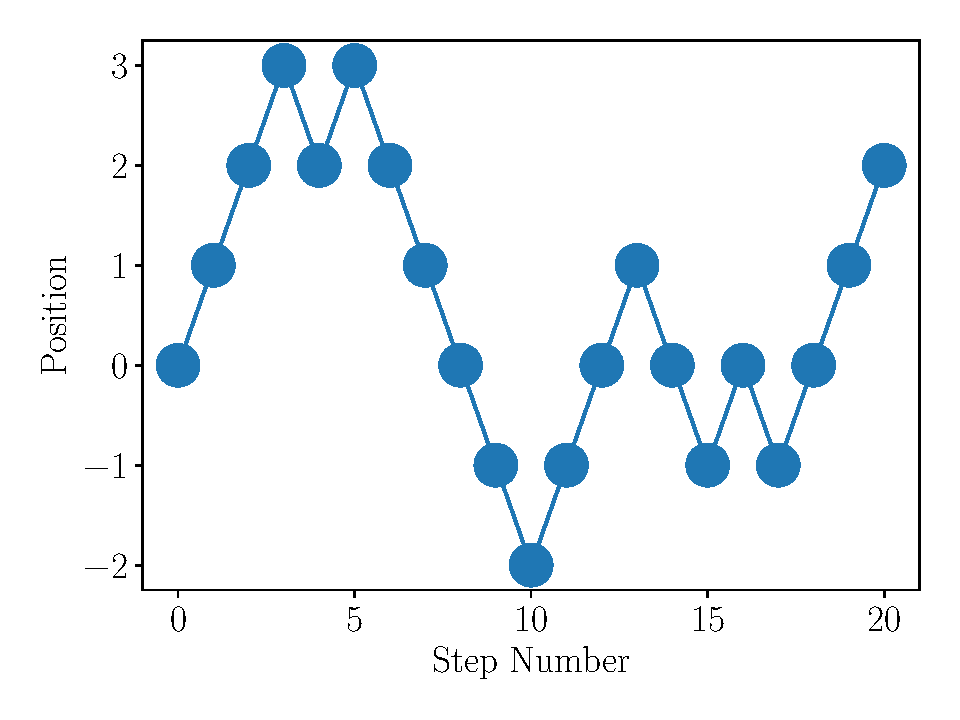
\includegraphics[width=0.45\textwidth]{images/cartoon.pdf}
    \caption{The position of a walker at each step in a 20-step random walk
      simulation. The average position of the walker does not necessarily remain
      at the origin as one might naively expect. Instead it is normal for the
      walker to finish the walk at some distance from the origin, as shown here.}
    \label{fig:cartoon}
  \end{center}
\end{figure}

As we can see from the figure, it is not uncommon for the average position of
the walker to be away from the origin once the walk has concluded. This is
because the position of the walker at any step is dependent only on the position
at the previous step. If the walker happens to take a number of steps in the
same direction, it is highly unlikely for the walker to take an equal number of
steps in the opposite direction, in order to return to the origin. Thus, in such
a case, it is likely that the walker will conclude the walk in a position away
from the origin.

In this example, the walker had an equal likelihood of stepping forward or
backwards, but we can bias in one way if we want to model a particular
phenomenon. The walk is also easily extensible to multiple dimensions, as for
each extra dimension, one extra random number must be drawn. This gives a linear
increase in time-complexity, which is convenient for more complex systems.

\subsection{Application to Quantum Systems}

This investigation applied Random walk simulations to calculate the ground state
energies of Quantum Systems by solving the Schr\"{o}dinger equation, as shown in
\todo{cite}.

We can extend the simple one-dimensional line model from Figure
\ref{fig:cartoon} to a quantum system by imagining it as a one-dimensional
simple lattice system. A walker can start at a position labelled the origin, and
then proceed in a random walk. The random walk concludes if the walker ``dies''
on a particular step. The probability that the walker will die is dependent on a
defined potential at that point. For example, in an infinite square well system,
the potential is 0 within a well, and infinite outside the well. So the walker
will have no chance of dying whilst inside the well, but will die if they step
outside.

Let us define $p(j,n)$ as the probability that the walker will be at position
$j$ after $n$ steps and $a(j)$ as the probability that the walker will die at
position $j$. Thus, for this to be the case, the walker would have had position
$j\pm1$ after $n-1$ steps. Thus, we can say:

\begin{equation}
  p(j, n+1) =  \frac{1}{2}(1-a(j))(p(j-1,n) + p(j+1,n))
  \nonumber
\end{equation}

If $a(j)$ is small and $n$ is large, we can use Taylor's expansion to expand
each term in this expression and obtain a differential equation. If we then
make the ansatz substitution:

\begin{equation}
  p(j,n) = q(j) \exp(-\lambda n)
  \label{eq:firsteq}
\end{equation}
where $q(j)$ is an arbitrary function and $\lambda$ is the rate of death, then
we find:

\begin{equation}
  -\frac{1}{2} \frac{d^2q(j)}{dj^2} + a(j)q(j) = \lambda q(j)
  \label{eq:randomwave}
\end{equation}
The full derivation is taken from \cite{MarcusNewton2020} and is shown in
Appendix \ref{appendix:derivation}. Notice that Equation \ref{eq:randomwave} is
in the form of the Schr\"{o}dinger equation:

\begin{equation}
  \label{eq:schrodinger}
  \frac{-\hbar^2}{2m}\frac{d^2 \psi}{dr^2} + V(r)\psi(r) = E\psi(r)
\end{equation}
Comparing Equation \ref{eq:randomwave} and Equation \ref{eq:schrodinger}, we can
see that the probability of death $a(j)$ is related to the potential $V(r)$,
and the rate of death $\lambda$ is related to the Energy $E$.

We can extend this to an infinite square well by choosing our probability of
death such that:

\begin{equation}
  \label{eq:squarewell}
    a(j) =
    \begin{cases}
      0,& \text{if } j < J\\
      \infty,& \text{if } j \geq J
    \end{cases}
    \nonumber
\end{equation}
where J is a well-defined boundary. So the walker cannot die inside the well but
wil immediately die when they step outside, which we expect will definitely
happen given sufficient time. Inside the well, the potential is simply that of a
free particle:

\begin{equation}
  \frac{-\hbar^2}{2m}\frac{d^2 \psi}{dx^2} = E\psi(x)
  \nonumber
\end{equation}
where $x$ is the position of the walker. By making the substitution
$x=J\frac{j}{R}$, such that $j=R$ corresponds to the walker being at the
boundary, we find:

\begin{equation}
  \begin{split}
    -\frac{\hbar^2}{2m}\frac{R^2}{J^2}\frac{d^2\psi}{dj^2} &= E\psi(x)\\
    -\frac{1}{2}\frac{d^2\psi}{dj^2} &= \frac{mJ^2E}{\hbar^2R^2}\psi(x)
  \end{split}
  \nonumber
\end{equation}
If we compare this to Equation \ref{eq:randomwave}, allowing $a(j) = 0$ inside
the well, we see that:

\begin{equation}
  E = \lambda R^2 \frac{\hbar^2}{mJ^2}
  \nonumber
\end{equation}
where only $\lambda$ is an unknown quantity. Thus, by calculating rate of death
$\lambda$, we can calculate the ground state energy of the infinite square
well. The known ground state energy of an infnite square well is
$\frac{\pi^2}{8}\frac{\hbar^2}{mJ^2}$ \todo{cite}, so we expect to find $\lambda
R^2$ close to $\frac{\pi}{8}$.


\section{Method}

The Random walk is implemented computationally \todo{cite} and is extensible
to multiple dimensions. For a $N$-dimensional lattice, at each point there are
$2N$ possible directions for the walker to move. So a direction is selected
randomly using a Mersenne Twister pseudorandom number generator (pRNG). This algorithm
was chosen as it is a very fast implementation of a pRNG \todo{cite} and it
passes many statistical randomness tests \todo{cite}, and has a very large
period of $2^{19937-1}$.

The random walk ends when a walker dies, with a
specifically chosen $a(j)$. Initially, the $a(j)$ is chosen to be that of an
infinite square well \todo{cite}, that is:
\begin{equation}
  \label{eq:squarewell}
    a(j) =
    \begin{cases}
      0,& \text{if } j < J\\
      \infty,& \text{if } j \geq J
    \end{cases}
    \nonumber
\end{equation}
where J is a well-defined boundary. So the walker has no chance of dying whilst
within the well, but will die immediately once reaching the boundary. As
explained in Section \ref{sec:TheoreticalBackground}, we expect that given
sufficient time, all the walkers will reach the boundary and die. But in order
to save computational resources, a maximum number of steps may also be defined,
such that a walker will also die should they move that number of steps without
reaching a boundary. This was not initially implemented, as it can introduce
systematic errors, since there would be a disproportionate number of walkers dying
on the maximum number of steps.

Thus, the Schr\"{o}dinger equation inside a one-dimensional infinite square well
is simply that of a free particle \todo{cite}:
\begin{equation}
  \frac{-\hbar^2}{2m}\frac{d^2 \psi}{dx^2} = E\psi(x)
  \nonumber
\end{equation}
where $x$ is the position of the walker. By making the substitution $x = J
\times j/R$, such that $j=R$ corresponds to the walker being at the boundary, we
obtain:
\begin{equation}
  \begin{split}
    -\frac{\hbar^2}{2m}\frac{R^2}{J^2}\frac{d^2\psi}{dj^2} &= E\psi(x)\\
    -\frac{1}{2}\frac{d^2\psi}{dj^2} &= \frac{mJ^2E}{\hbar^2R^2}\psi(x)
  \end{split}
  \nonumber
\end{equation}

If we compare this to Equation \ref{eq:randomwave}, allowing $a(j) = 0$ inside
the well, we see that:
\begin{equation}
  \begin{split}
    \lambda &= \frac{mJ^2E}{\hbar^2R^2} \\
    E &= \lambda R^2 \frac{\hbar^2}{mJ^2}
  \end{split}
  \nonumber
\end{equation}

So, by calculating the death rate $\lambda$, we can find the ground state energy
of a particle in an infinite square well.

But the known ground state of a particle in an infinite square well is
$\frac{\pi^2}{8}\frac{\hbar^2}{mJ^2}$ \todo{cite}. This implies that we expect $\lambda
R^2=\frac{\pi^2}{8}$ where R is the boundary of the well. Thus, we expect to
find a $\lambda$ that is close to this theoretical value.


To find the rate of death $\lambda$, we consider Equation \ref{eq:firsteq}. With
some simple manipulation:
\begin{equation}
  \begin{split}
    p(j, n) & = q(j) \exp(-\lambda n)\\
    \log(p) & = \log(q \exp(-\lambda n)) \\
  \end{split}
  \nonumber
\end{equation}

\begin{equation}
  \log(p) = -\lambda n + log(q)
  \label{eq:straightline}
\end{equation}

Thus, by plotting the logarithm of the probability of surviving $n$ steps
against the number of steps $n$, we can obtain the death rate $\lambda$ from the
gradient.

Varying the boundary $J$ of the square well will affect the accuracy of the
final answer, and this is also investigated here.


\section{Results and Discussion}
The simulation was first run for an infinite square well with boundary $J = 20$,
with 1000000 walkers. The step on which each walker died was recorded and then
the normalised histogram in Figure \ref{fig:hist} was constructed. The histogram
has been normalised, and is hence a probability distribution showing the
probability that a walker will die on a particular step. As we expect, the peak
is far from the origin, since for a walker to die in an inifinite square well
with $J=20$, they would have to walk at least 20 steps. It is also highly
unlikely that a walker would walk 20 steps in the same direction
consecutively. Thus, the peak is also at a number of steps greater than $J$. We
expect the shape of the decay after the peak to be exponential. We can see this
by plotting the histogram on a logarithmic scale.

Figure \ref{fig:loghist} presents the same histogram data with a logarithmic y
scale. In this figure, a straight line is evident in the data, showing the decay
was indeed exponential after the peak. The peak probability being away fro the
origin is also clearer in this figure. Figure \ref{fig:loghist} shows a
``widening'' of the straight line at higher step numbers. This is because there
is a greater variance in the number of walkers surviving to this number as it is
highly unlikely. 

By taking the cumulative sum of the histograms in Figure \ref{fig:expplots}, we
can ensure the peak probability begins at the origin. Figure \ref{fig:cumplots}
present the cumulative sums of the histograms. They represent the probability of
surviving at least a particular number of steps. Hence, the peak probability of
1 is at the origin, since there is a probability of 1 that a walker will survive
the first step.

Figure \ref{fig:cumhist} presents the cumulative summed histogram, with a fitted
exponential curve of the form of Equation \ref{eq:firsteq}. The fit is very
good, with $R^2 = 0.9999998$, very close to 1. There is also negligible
numerical error in the fit, i.e. an error smaller than the quoted precision of
the fit parameters. This is because the simulation was run for 1000000 walkers,
providing a large sample size. Figure \ref{fig:cumloghist} presents the same
histogram with a logarithmic y-scale and a fitted straight line of the form of
Equation \ref{eq:straightline}. This fit has the same $R^2$ value, as it is
simply the same fit on a different y-scale, and is thus equally good.

We observe some fluctuation in the data in the higher steps. This is because
there are so few walkers surviving to this many steps that there is more
significant variance in their relative numbers. It is possible to remove this
variance by introducing a cutoff number of steps, i.e. a maximum number of steps
at which the walker will automatically die, regardless of whether they reached a
boundary or not. Thus, there will not be such high variance in the number of
walkers surviving to high number of steps. This is presented in Figure
\ref{fig:cum_line_cutoff_plot}. While this fit is observed to be better, with a
higher $R^2$ value, some systematic error has been introduced since there will now
be a disproportionately high number of walkers dying at the cutoff step. Thus,
the final $\lambda J^2$ value will be less accurate. On a faster computer, with
more efficient code, it is possible to forgo the step cutoff and allow the
simulation to run until all the walkers die. This may take much longer but will
ensure there will not be such a systematic error introduced.

We can use the gradient of the fitted line in Figure \ref{fig:cumloghist} as the
$\lambda$ value, and compare $\lambda J^2$ with the theoretical value. However,
to determine the reliability of the calculated value, it is necessary to repeat
the procedure many times and take the average $\lambda$ and the standard
deviation as the error.

It is also necessary to investigate how varying the boundary $J$ affects the
accuracy of the final answer. Figure \ref{fig:multi_line_plot} presents the
cumulative summed histograms with their fitted lines for many different boundary
$J$ values. No step cutoff was introduced. The calculated $\lambda J^2$ value is
shown in the legend. \todo{truncate numbers} As shown, the gradient changes, but
this is to be expected since the expected highest number of steps would increase
as the boundary is larger, since there is more ``space'' for the walker to move
before reaching a boundary. As shown in the legend, the calculated $\lambda J^2$
values get closer and closer and closer to the theoretical value as $J$
increases. This is due to the fact that as $J$ increases, there are more walkers
surviving to larger number of steps. \todo{make plot of lambda J against J}.
Thus, we can say that using a larger value of $J$ will result in a more
accurate answer but will also be more computationally intensive and take
longer. Thus, we make a tradeoff between speed and accuracy and choose $J=20$
for the final investigation.

Running the simulation 10 times and taking the average $\lambda J^2$ with error
being standard deviation, we find: $\lambda J^2 = 1.2339 \pm 0.0008$. We quote
the precision to the decimal place at which there is variation from the
theoretical result of $1.2337$. We notice also that the error in the calculated
answer is small (since there is not much variation between repeated simulations)
and the theoretical result is within the range of the calculated answer.

\todo{circular well}
\begin{figure*}%[ht!]
  \centering
  \subfloat[Histogram of probability of dying on particlar step]
  {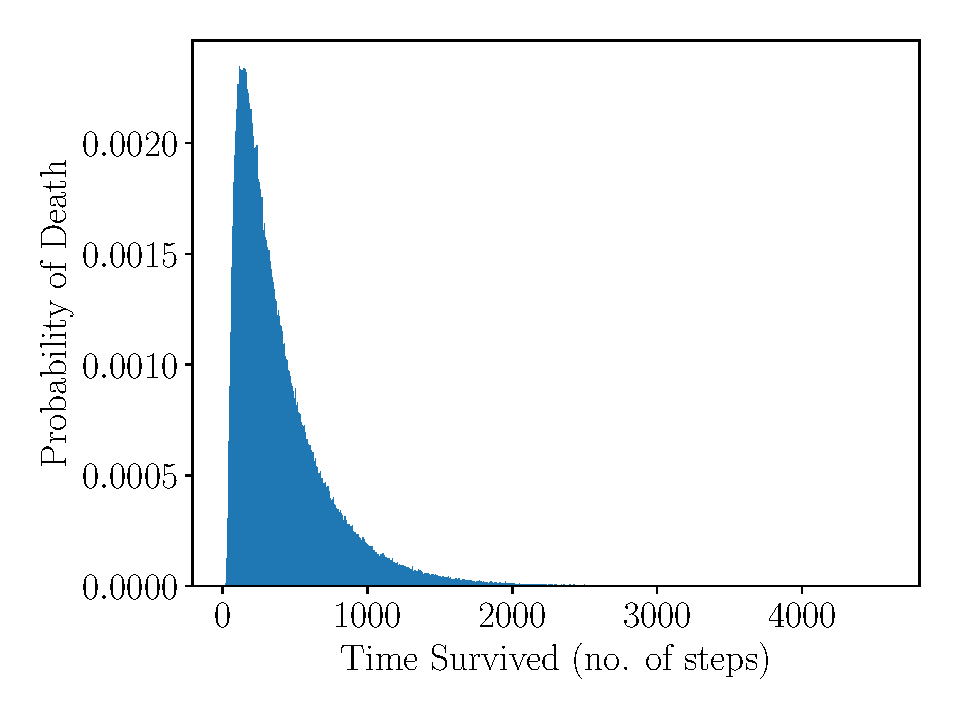
\includegraphics[width=0.5\textwidth]{images/exp_plot.pdf}
  \label{fig:hist}}
  \centering
  \subfloat[Histogram of probability of dying on particular step in a logarithmic scale]
  {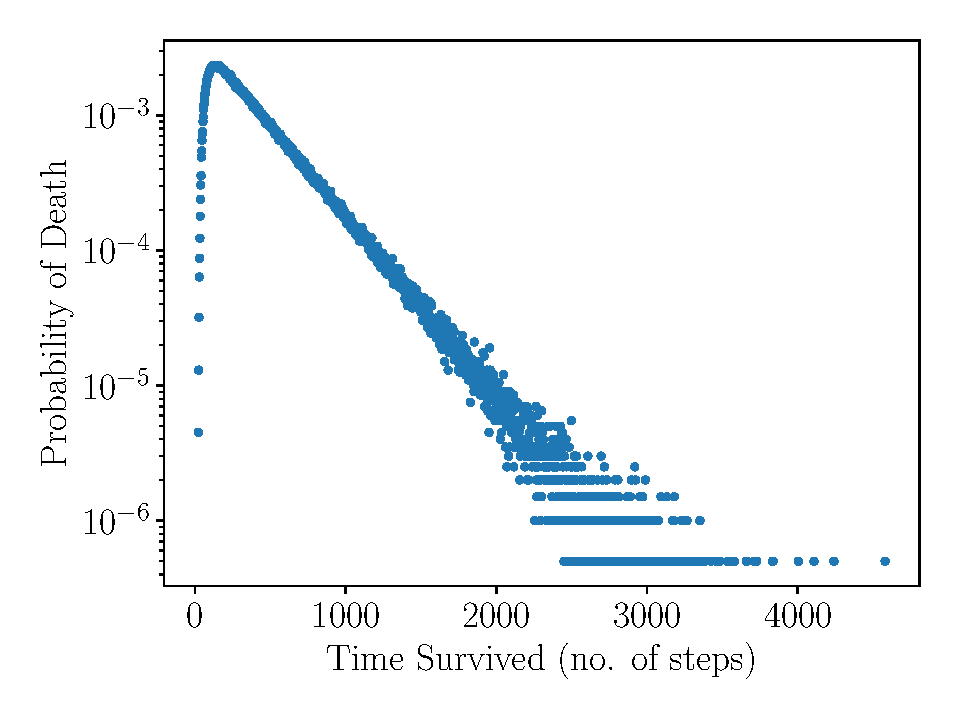
\includegraphics[width=0.5\textwidth]{images/line_plot.pdf}
    \label{fig:loghist}}
  \caption{Histograms showing the Probability of dying on a particular step in
    an infinite square well with $J = 20$. As can be seen, the peak is away from the
    origin, as is expected since it is not likely for a walker to die on a step $n$
    where $n < J$. The exponential decay after the peak is evident, implying a
    straight line shape if plotted on a logarithmic scale, which can be seen on
    the right hand side plot. In this logarithmic scale plot, the peak being away
    from the origin is clearer.}
  \label{fig:expplots}
\end{figure*}



\begin{figure*}%[ht!]
  \centering
  \subfloat[Histogram of probability of surviving to at least a particlar step]
  {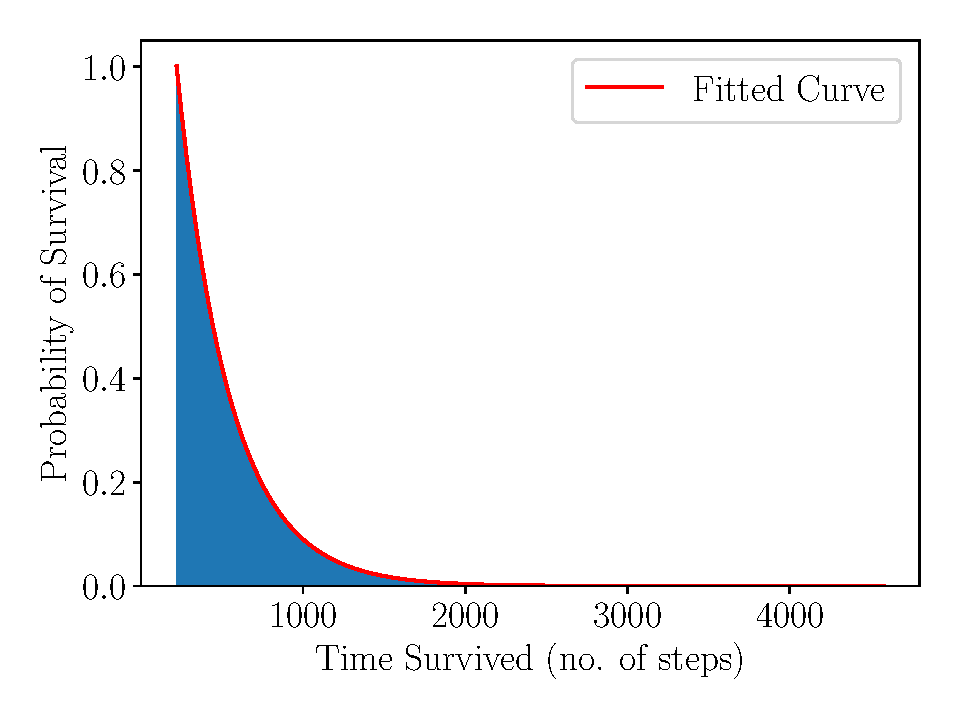
\includegraphics[width=0.5\textwidth]{images/cum_exp_plot.pdf}
  \label{fig:cumhist}}
  \centering
  \subfloat[Histogram of probability of surviving to at least a particular step
  in a logarithmic scale]
  {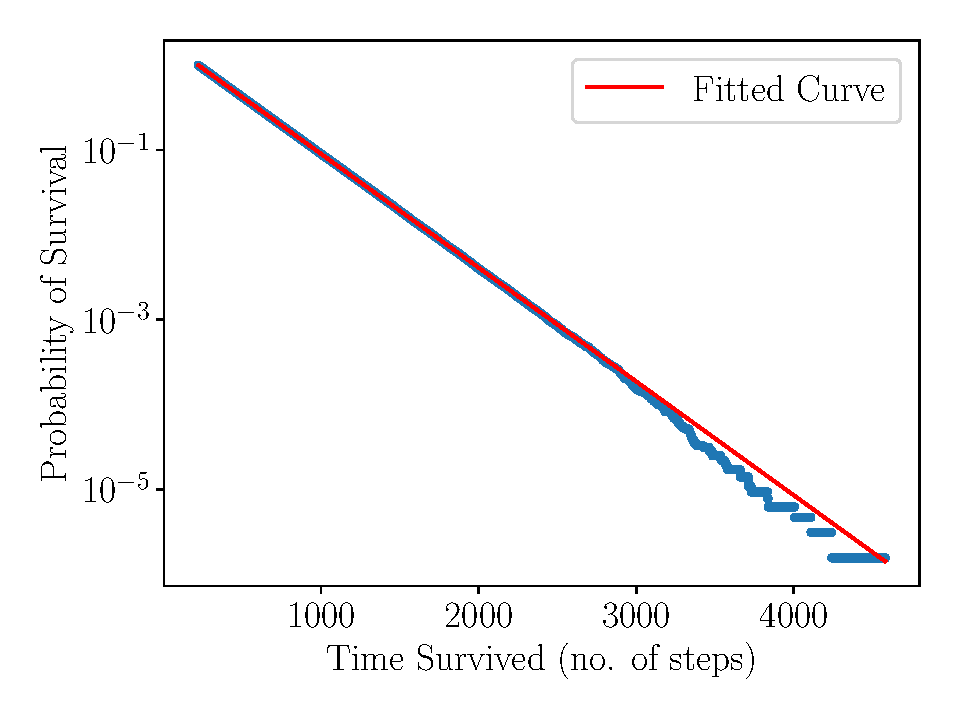
\includegraphics[width=0.5\textwidth]{images/cum_line_plot.pdf}
  \label{fig:cumloghist}}
  \caption{Histogram showing the Probability of surviving to at least a
      particular step in an infinite square well with $J = 20$. This is a
      cumulative sum of the bins in Figure \ref{fig:hist}. As can be seen, the
      peak is at the origin, since it is certain that no walker will die on the
      first step. An exponential decay curve provides a good fit, with an $R^2$
      value of 0.9999998, very close to 1. Plotting on a logarithmic scale shows
      the straight line fit, the gradient of which is $\lambda$, giving $\lambda
      J^2 = 1.2334$, with a negligible error.}
  \label{fig:cumplots}
\end{figure*}

\todo{fix centering of cum plot}

\begin{figure}%[!ht]
  \begin{center}
    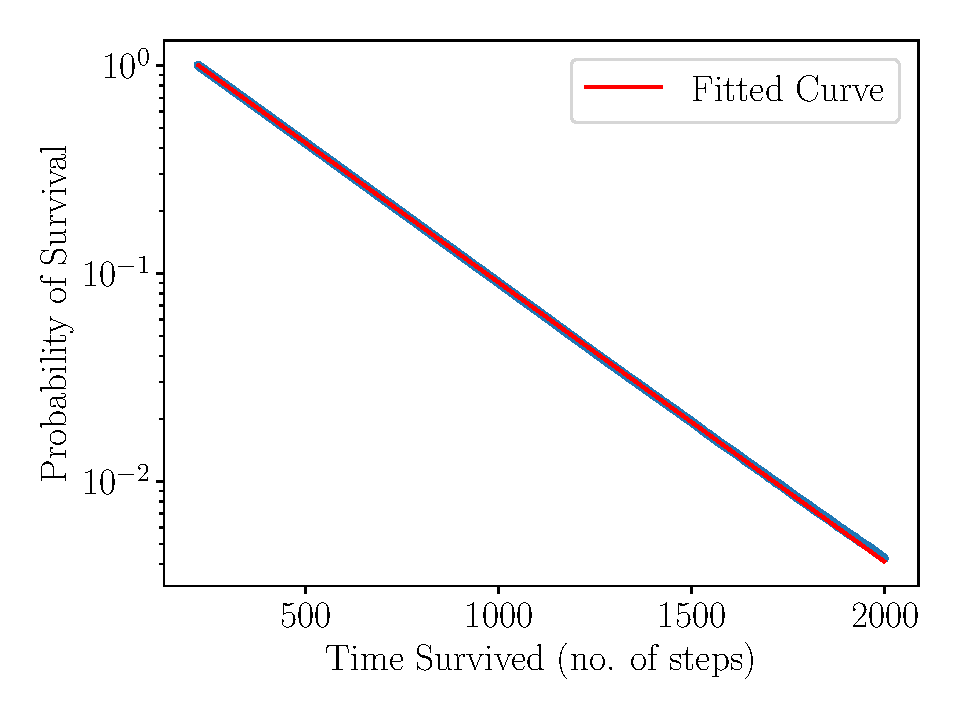
\includegraphics[width=0.45\textwidth]{images/cum_line_plot_cutoff.pdf}
    \caption{Histogram plotted on a logarithmic scale showing the Probability of
      surviving to at least a particular step in an infinite square well with $J
      = 20$, and also introducing a maximum number of steps at 2000, after which
      all walkers will die. This saves computational resources but introduces
      some systematic error, as there will now be a disproportionately high
      number of walkers in the 2000 steps bin.}
    \label{fig:cum_line_cutoff_plot}
  \end{center}
\end{figure}


\begin{figure}%[!ht]
  \begin{center}
    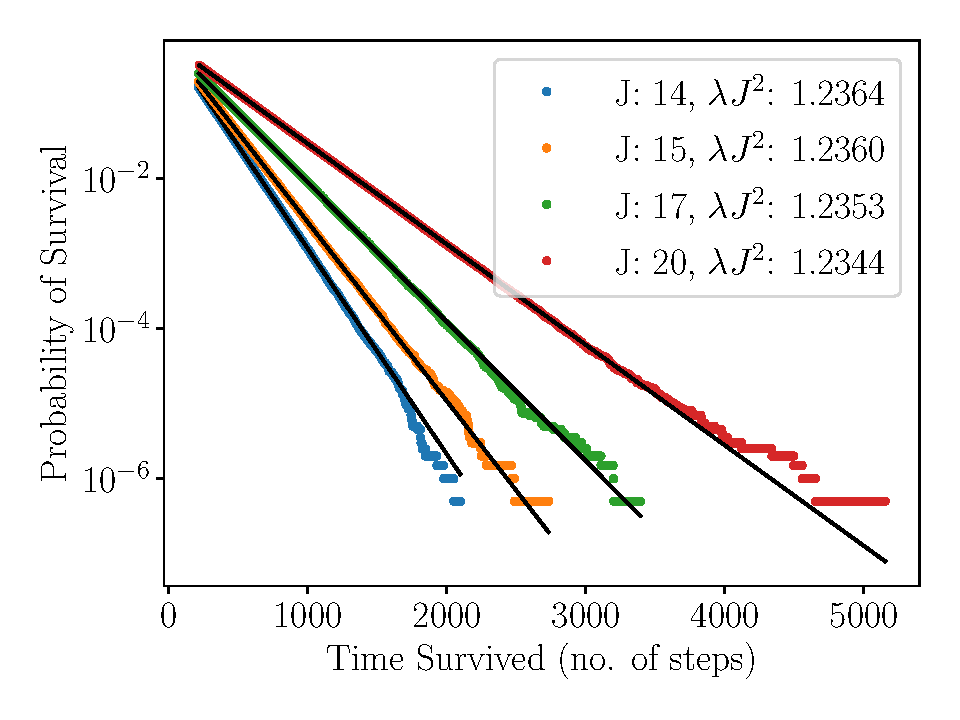
\includegraphics[width=0.45\textwidth]{images/multiplot.pdf}
    \caption{Histogram plotted on a logarithmic scale showing the Probability of
      surviving to at least a particualr step in different infinite square wells with
      different boundaries $J$. The $\lambda J^2$ values for each are shown. The
      values get closer to the theoretical value of $\frac{\pi^2}{8}$ as we increase
      the size of the well. This is likely due to more walkers surviving to a higher
      number of steps, as the well size is increased.}
    \label{fig:multi_line_plot}
  \end{center}
\end{figure}


\section{Conclusions}

In this investigation we demonstrated a method of calculating ground state
energies of a quantum system using Random walk computational simulations. The
investigation focussed on an Infinite Square Well, but is easily extended to a
Symmetric potential. The simualation was written in C++ to maximise performance
and is available at \todo{cite}.

The investigation explored the effects of varying the size of the well in
determining the ground state energy of a quantum system, and showed that this
method is more effective for larger wells, i.e. wells with larger
boundaries. This is because for wells with larger boundaries, the walker can
take a larger number of steps on average before dying, and thus can populate
larger step bins. Thus, this method produces data that is close to the
theoretical result for larger infinite square wells.

The general theoretical result for the ground state energy of an infinite square
well is $\frac{\pi^2}{8}\frac{\hbar^2}{mJ^2}$ where $J$ is the boundary of the
well, and this method allows for the calculation of $\lambda R^2
\frac{\hbar^2}{mJ^2}$, where $R$ also corresponds to the boundary of the
well. Thus, we expect our calculated result to be $\lambda R^2 = \lambda J^2 =
\frac{\pi^2}{8}$.

This method provided $\lambda J^2 = 1.2339 \pm 0.0008$, which lies within the
range of the theoretical result.

This method can be easily extended to multiple dimensions with only a linear
increase in time complexity for each added dimension. Thus, while this method
may not be very efficient for low number of dimensions, it quickly becomes
effective at a higher number of dimensions.



% if have a single appendix:
%\appendix[Proof of the Zonklar Equations]
% or
%\appendix  % for no appendix heading
% do not use \section anymore after \appendix, only \section*
% is possibly needed

% use appendices with more than one appendix
% then use \section to start each appendix
% you must declare a \section before using any
% \subsection or using \label (\appendices by itself
% starts a section numbered zero.)
%



\appendices
\section{Random walk Schr\"{o}dinger Equation Derivation}
\label{appendix:derivation}
Let us denote the probability that the walker is at position $j$ after $n$ steps
as $p(j,n)$ and the probabilty that the walker will die at position $j$ as
$a(j)$. We will denote the position-step number coordinates as $[j, n]$. Thus,
for a walker to have coordinates $[j, n+1]$, in the previous step, they must have
had coordinates $[j \pm 1, n]$. So we can say:

\begin{equation}
  \label{eq:probability}
  p(j, n+1) =  \frac{1}{2}(1-a(j))(p(j-1,n) + p(j+1,n))
\end{equation}

If $a(j)$ is small and $n$ is large, then we can say $p(j, n)$ is a continuous
function and we can use Taylor expansion to expand each of $p(j+1, n)$,
$p(j-1,n)$, and $p(j, n+1)$:

\begin{equation}
  p(j+1, n) = p(j,n) + \frac{\partial p}{\partial j} + \frac{1}{2}
  \frac{\partial^2 p}{\partial j^2} + ...
  \nonumber
\end{equation}
\begin{equation}
  p(j-1, n) = p(j,n) - \frac{\partial p}{\partial j} + \frac{1}{2}
  \frac{\partial^2 p}{+\partial j^2} + ...
  \nonumber
\end{equation}
\begin{equation}
  p(j, n+1) = p(j, n) + \frac{\partial p}{\partial n} + ...
  \nonumber
\end{equation}

We can now substitute these expansions into Equation \ref{eq:probability}, we
find:

\begin{equation}
  p(j, n) + \frac{\partial p}{\partial n} = (1-a(j))\Big(p +
  \frac{1}{2}\frac{\partial^2 p}{\partial j^2}\Big)
  \nonumber
\end{equation}

But the probability of death $a(j)$ and the second derivative are so small, that
their product is neglected. We also let $p(j,n) = q(j) \exp(-\lambda n)$ so that:

\begin{equation}
  -\frac{1}{2} \frac{d^2q(j)}{dj^2} + a(j)q(j) = \lambda q(j)
  \nonumber
\end{equation}

\printbibliography

\end{document}


